\documentclass[10pt,conference,compsocconf]{IEEEtran}

\usepackage{hyperref}
\usepackage{graphicx}	% For figure environment


\begin{document}
\title{Machine Learning Report}

\author{
  Raphael Barman, Hakim Invernizzi, Rehan \\
  \textit{EPFL students}
}

\maketitle

\begin{figure}
\begin{center}
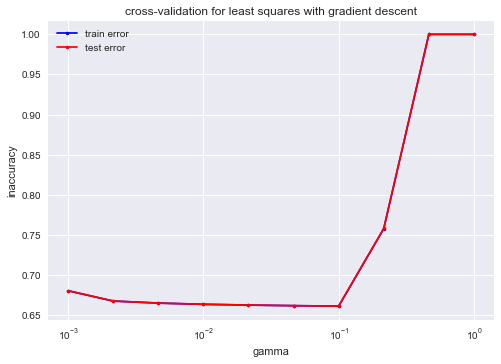
\includegraphics[width=4.5cm]{cross_validation_least_squares_GD.png}
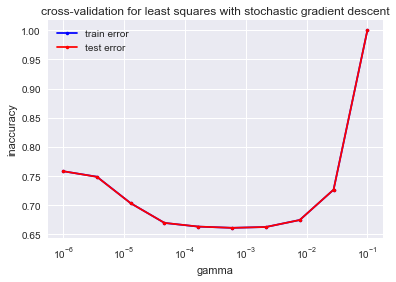
\includegraphics[width=4.5cm]{cross_validation_least_squares_SGD.png}
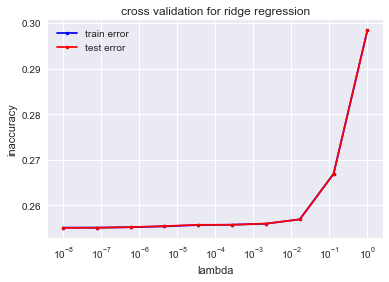
\includegraphics[width=4.5cm]{cross_validation_ridge_regression.png}
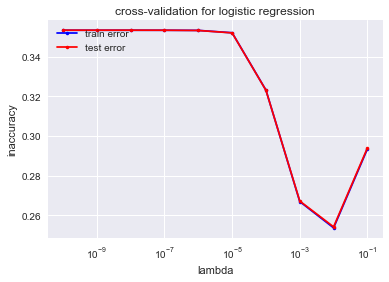
\includegraphics[width=4.5cm]{cross_validation_logistic_regression.png}
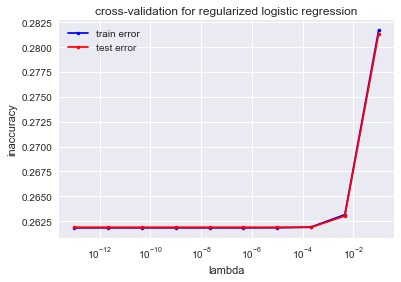
\includegraphics[width=4.5cm]{cross_validation_reg_logistic_regression.png}
 \end{center}
 \begin{center}
 \caption{\label{fig:figure1}Result of Cross-Validation with 10 folds. On the X-axis we have the ML method parameter to be tuned, on the Y-axis a measure of the inaccuracy. From top to bottom: (a) least squares GD (b) least squares GD (c) ridge regression (d) logistic regression (e) logistic regression with regularization}
 \end{center}
\end{figure}

\section{Part I: Machine learning methods implementation}
Here is the description of our implementation of the six machine learning methods.\\
Please note that we defined our own metric to estimate prediction error, which is not the MSE but simply the percentage of uncorrectly predicted outputs, which we call inaccuracy. 
This metric is used exclusively to evaluate performance and isn't part of the implementation.
 \subsection{Linear regression using gradient descent}
The implementation is simple: we iteratively update the initial weight by subtracting a pondered gradient.
\ref{fig:figure1} (a) shows the method gives around 66\% inaccuracy in the best case, and performs best when gamma is on the order of $10^{-1}$. 
\subsection{Linear regression using stochastic gradient descent}
The difference compared to the previous method is that at each iteration the dataset is accessed at random indexes in order to
create size-1 batches. The batch gradient is then computed, pondered and used to update the weight.
\ref{fig:figure1} (b) shows the method gives 26\% inaccuracy in the best case, and performs best when gamma is on the order of $10^{2}$. 
\subsection{Least squares regression}
The pseudo-inverse of the feature matrix \textit{tx} is computed and then multiplied with the classification vector \textit{y} to obtain the weight.
The inaccuracy is of around 25.5\% for both train and test dataset.
\subsection{Ridge regression}
The weight is computed by solving the ridge regression equation, yielding $w = (X^{T}X + \lambda'I)^{-1}X^{T}y$.
\ref{fig:figure1} (c) shows that the performance of the ridge regression is comparable to that of the simple least square regression, suggesting that regularisation applied to the whole dataset provides little improvement.
\subsection{Logistic regression}
//describe
\ref{fig:igure1} (d) shows the method gives around 25.7 \% inaccuracy in the best case
\subsection{Regularized logistic regression}
//describe
\ref{fig:figure1} (b) shows the method gives 26.25\% inaccuracy in the best case, reinforcing what previously said about regularization.
\section{Our Model}
\subsection{Exploratory Data Analisis and Feature Processing}
EDA produces the following observations:

The training dataset can be divided in six groups based on the entry values of feature 0 and 22. These six highly intra-correlated group are treated separately in the subsequent operations.

Features 15, 18, 20, 25 and 28 don't provide useful information because the distribution of both type of particles (s and b) based on these feature is  identically uniform.

Features 0, 1, 2, 3, 5, 8, 9, 10, 13, 19, 21, 23, 26 and 29 follow an exponential distribution and are therefore standardized before being used in the ML method.
\subsection{ML method and Cross-validation}
The chosen ML method is Ridge Regression because it has the lowest inaccuracy among the six baseline methods.
The tuning of the model consisted of a process of iterative cross-validation applied to Ridge Regression, with and without making use of extended feature vectors.
This allowed to find the following optimal polynomial degrees and lambda values for each of the six groups:
$(d_0 = 4, \lambda_0 = 0.031)$
$(d_1 = 5, \lambda_1 = 1e-10)$
$(d_2 = 6, \lambda_2 = 1.29e-9)$
$(d_3 = 5, \lambda_3 = 0.00046)$
$(d_4 = 7, \lambda_4 = 0.00316)$
$(d_5 = 3, \lambda_5 = 2.78255e-6)$

\end{document}
